\pgfdeclaredecoration{discontinuity}{start}{
  \state{start}[width=0.5\pgfdecoratedinputsegmentremainingdistance-0.5\pgfdecorationsegmentlength,next state=first wave]
  {}
  \state{first wave}[width=\pgfdecorationsegmentlength, next state=second wave]
  {
    \pgfpathlineto{\pgfpointorigin}
    \pgfpathmoveto{\pgfqpoint{0pt}{\pgfdecorationsegmentamplitude}}
    \pgfpathcurveto
        {\pgfpoint{-0.25*\pgfmetadecorationsegmentlength}{0.75\pgfdecorationsegmentamplitude}}
        {\pgfpoint{-0.25*\pgfmetadecorationsegmentlength}{0.25\pgfdecorationsegmentamplitude}}
        {\pgfpoint{0pt}{0pt}}
    \pgfpathcurveto
        {\pgfpoint{0.25*\pgfmetadecorationsegmentlength}{-0.25\pgfdecorationsegmentamplitude}}
        {\pgfpoint{0.25*\pgfmetadecorationsegmentlength}{-0.75\pgfdecorationsegmentamplitude}}
        {\pgfpoint{0pt}{-\pgfdecorationsegmentamplitude}}
}
\state{second wave}[width=0pt, next state=do nothing]
  {
    \pgfpathmoveto{\pgfqpoint{0pt}{\pgfdecorationsegmentamplitude}}
    \pgfpathcurveto
        {\pgfpoint{-0.25*\pgfmetadecorationsegmentlength}{0.75\pgfdecorationsegmentamplitude}}
        {\pgfpoint{-0.25*\pgfmetadecorationsegmentlength}{0.25\pgfdecorationsegmentamplitude}}
        {\pgfpoint{0pt}{0pt}}
    \pgfpathcurveto
        {\pgfpoint{0.25*\pgfmetadecorationsegmentlength}{-0.25\pgfdecorationsegmentamplitude}}
        {\pgfpoint{0.25*\pgfmetadecorationsegmentlength}{-0.75\pgfdecorationsegmentamplitude}}
        {\pgfpoint{0pt}{-\pgfdecorationsegmentamplitude}}
    \pgfpathmoveto{\pgfpointorigin}
}
  \state{do nothing}[width=\pgfdecorationsegmentlength,next state=do nothing]{
    \pgfpathlineto{\pgfpointdecoratedinputsegmentlast}
  }
  \state{final}
  {
    \pgfpathlineto{\pgfpointdecoratedpathlast}
  }
}



\tikzset{%
  neuron missing/.style={
    draw=none, 
    scale=4,
    text height=0.333cm,
    execute at begin node=\color{black}$\vdots$
  },
}
\hspace*{1cm}
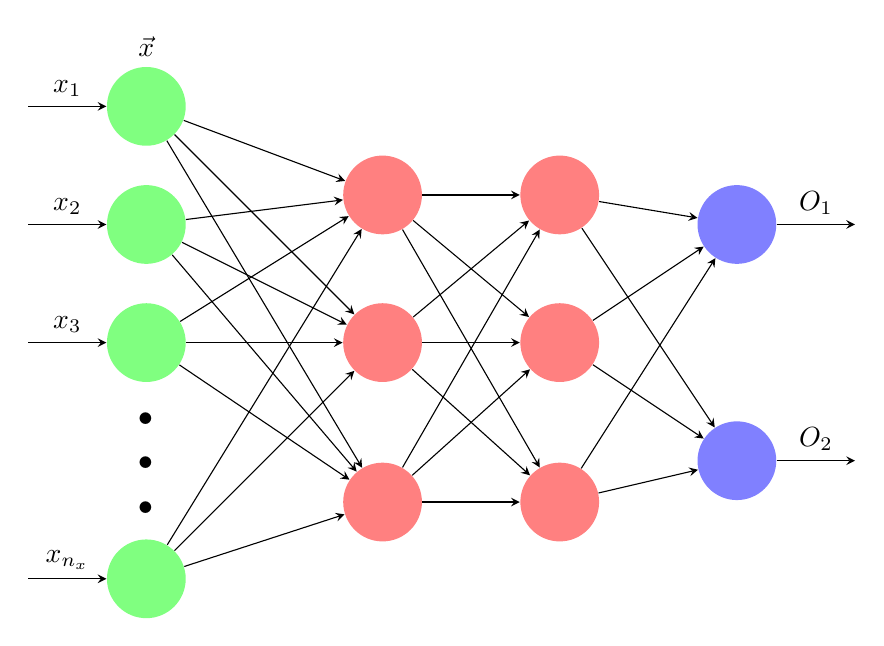
\begin{tikzpicture}[x=1.5cm, y=1.5cm, >=stealth]
  % draw input features  
  \foreach \m/\l [count=\y] in {1,2,3}
  {
    \node [circle,fill=green!50,minimum size=1cm] (input-\m) at (0,2.5-\y) {};
  }
  \foreach \m/\l [count=\y] in {4}
  {
    \node [circle,fill=green!50,minimum size=1cm ] (input-\m) at (0,-2.5) {};
  }
  
  \node [neuron missing]  at (0,-1.5) {};
  % draw hidden layers
  %first hidden layer
  \node [circle,fill=red!50,minimum size=1cm ] (hidden1-1) at (2,0.75) {};
  \node [circle,fill=red!50,minimum size=1cm ] (hidden1-2) at (2,-0.5) {};
  \node [circle,fill=red!50,minimum size=1cm ] (hidden1-3) at (2,-1.85) {};  
  %second hidden layer
  \node [circle,fill=red!50,minimum size=1cm ] (hidden2-1) at (3.5,0.75) {};
  \node [circle,fill=red!50,minimum size=1cm ] (hidden2-2) at (3.5,-0.5) {};
  \node [circle,fill=red!50,minimum size=1cm ] (hidden2-3) at (3.5,-1.85) {};  

  % draw output neurons
  \node [circle,fill=blue!50,minimum size=1cm ] (output-1) at (5,0.5) {};
  \node [circle,fill=blue!50,minimum size=1cm ] (output-2) at (5,-1.5) {};

  \foreach \l [count=\i] in {1}
  \node [above] at (input-\i.north) {$\vec{x}$};

  \foreach \l [count=\i] in {1,2,3,n_x}
  \draw [<-] (input-\i) -- ++(-1,0)
  node [above, midway] {$x_{\l}$};


  \draw [->] (output-1) -- ++(1,0)
  node [above, midway] {$O_{1}$};
  \draw [->] (output-2) -- ++(1,0)
  node [above, midway] {$O_{2}$};

  \foreach \i in {1,...,4}
  \foreach \j in {1,...,3}
  \draw [->] (input-\i) -- (hidden1-\j);

  \foreach \i in {1,2,3}
  \foreach \j in {1,2,3}
  \draw [->] (hidden1-\i) -- (hidden2-\j);
  
  \foreach \i in {1,2,3}
  \foreach \j in {1,2}
  \draw [->] (hidden2-\i) -- (output-\j);
  
  % \foreach \l [count=\x from 0] in {Input, Hidden, Ouput}
  % \node [align=center, above] at (\x*2,2) {\l \\ layer};

\end{tikzpicture}
